\documentclass[oneside,12pt]{report}
\usepackage{graphicx} % To insert images
\usepackage{graphicx} % Required for inserting images
\usepackage{amsmath} % For advanced math commands
\usepackage{amsfonts} % For math fonts
\usepackage{amssymb} % For additional symbols
\usepackage{float}  % Add this package for the [H] specifier
\usepackage{amstext}
\usepackage{ragged2e}
\usepackage{enumitem}
\usepackage{glossaries}
\usepackage[left=2.5cm,right=2cm,top=2.5cm,bottom=2cm]{geometry}
\usepackage[skip=10pt plus1pt, indent=40pt]{parskip}
\usepackage{hyperref} % for referencing
\hypersetup{
    colorlinks=true,
    linkcolor=black,
    citecolor=black,
    filecolor=magenta,      
    urlcolor=blue,
    pdftitle={Overleaf Example},
    pdfpagemode=FullScreen,
    }
\usepackage{microtype}
\justifying
\begin{document}

\thispagestyle{empty}
	
	\begin{center}

		{\huge \textbf{Coalition Formation Using Lanchester Model: Including Internal and External Stability between two coalitions} \par}
	\vspace{2cm}

	{\LARGE \textbf {Project Seminar Report}  \par}
        {\Large \textbf {June, 2024} \par}
	\vspace{1.2cm}

        {\large Submitted By:\par}
	{\Large \textbf {Rupeshkumar Kanpariya(222202556)} \par}
        {\Large \textbf {Paras Bhalala(222202629)} \par}
        {\Large \textbf {Dharmik Dave(222201616)} \par}
	\vspace{0.8cm}
 
	{\large Guided By:\par}
	{\Large \textbf {Dr. Radomir Pestow} \par}
	\vspace{2cm}

        {\Large \textbf {Department of Mathematics,}\par}
        {\Large \textbf {Universität Koblenz}\par}
        \vspace{0.5cm}
	\begin{figure}[h]
		\centering
		\includegraphics[width=0.5\linewidth]{Images/logo.pdf}
		\label{fig:uk-fb3-logo-cmyk}
	\end{figure}
	\end{center}


\newpage
 \pagenumbering{roman}
	\pagestyle{plain}

	\section*{Declaration}
	\vspace{0.5cm}
		{We hereby declare that our project report entitled "Coalition Formation Using Lanchester Model: Including Internal and External Stability between two coalitions” is our original work submitted in partial fulfilment of the  "Mathematical Modeling, Simulation, and Optimization”. All sources of information, including but not limited to literature, data, and ideas, have been appropriately cited and referenced in accordance with academic standards and guidelines. This report represents the findings and conclusions based on our research and analysis in the field of Coalition Formation Using Lanchester Model: Including Internal and External Stability between two coalitions.  \par}
		
		
\vspace{1cm}
\begin{flushright}
Rupeshkumar Kanpariya - (Author \& Illustrator) (222202556) \par
Paras Bhalala - (Co-Author \& Programmer) (222202629) \par
Dharmik Dave - (Researcher) (222201616) \par
\vspace{1cm} 
 Date: 24 July, 2024 \par
\end{flushright}


\newpage
 
\section*{Acknowledgment}
\vspace{0.5cm}
We extend our heartfelt gratitude to our guide Dr. Radomir Pestow, for his invaluable mentorship, support, and expert guidance throughout this project. His extensive expertise and constructive feedback played a pivotal role in shaping the trajectory of our research and fine-tuning our methodological approaches. Lastly, we appreciate the Department of Mathematics, Universität Koblenz for providing us the opportunity to be a part of such research project.


\newpage

\section*{Abstract}
\vspace{0.5cm}

This study explores the application of the Lanchester model to coalition formation, focusing on the dynamics of internal and external stability in competitive scenarios. Understanding how coalitions form, and achieve stability. In this paper, we determine the conditions under which coalitions win, achieve internal stability, and maintain external stability using the Lanchester model. Some parameters like kill rates, synergy effects, and stability conditions are analyzed to understand the dynamics of coalition formation and performance. The Balance of Power theory explains the interactions and relationships between countries in the global arena. In an international system without a central authority, each country's primary aim is to ensure its own survival.

\textbf{Keywords:} Lanchester Model, Coalition Formation, Balance of Power Theory


\tableofcontents
\listoffigures
\listoftables

\newpage
\newlist{abbrv}{itemize}{1}
\setlist[abbrv,1]{label=,labelwidth=1in,align=parleft,itemsep=0.1\baselineskip,leftmargin=!}

\chapter*{List of Abbreviations}
\chaptermark{List of Abbreviations}

\begin{abbrv}
\item[MAD]			Mutually Assured Destruction
\item[MAS]			Mutually Assured Stability
\end{abbrv}

\newpage

\pagenumbering{arabic} 

\chapter{Introduction}

The Lanchester model, named after its creator Frederick William Lanchester, is a mathematical model designed to describe combat dynamics between opposing forces. Lanchester, an English engineer and mathematician, first introduced his model in 1916 during World War I \cite{r2}. Lanchester has developed two primary models to describe different types of combat:
\\[2em]
\textbf{Lanchester's Linear Law:}
This Lanchester's Linear Law works in only close combat situations of ancient and medieval warfare, for example, infantry, cavalry, archers and more. The equations of the model are below: \cite{r8}

\begin{equation}
\frac{dA}{dt} = -\ k_b B A
\end{equation}

where A and B both are the army base or army size of coalition A and coalition B respectively, \(k_b\) is the kill rate of army of coalition B.

This above equation represents the rate at which the size of coalition A changes over time due to losses in battle. The term \(dA/dt\) indicates how the coalition A is losing its army and the negative sign signifies that the army of coalition A is decreasing over time. The rate of this decrease is directly proportional to the number of army in coalition B. This means that if there are more soldiers in coalition B, then coalition A will lose its army faster. In addition, the rate of loss for coalition A's army is also proportional to its own army size or army base (A). Here, \(k_b\) denotes the effectiveness of coalition B's attacks against coalition A.

\begin{equation}
\frac{dB}{dt} = -\ k_a A B
\end{equation}

where \(k_a\) is the effectiveness of army of coalition A.

This equation shows how the size of coalition B's army changes over time because of losses in battle. Here, \(dB/dt\) represents how coalition B is losing soldiers. The negative sign means that coalition B's army is getting reduced. The rate of this decrease depends on the number of soldiers in coalition A. So, if coalition A has more soldiers, coalition B will lose its soldiers faster. Also, the rate at which coalition B losses soldiers depends on the size of its own army. The constant \(k_a\) represents how effective coalition A's attacks are against coalition B.
\\[2em]
\textbf{Lanchester's Square Law:}
Generally, this model is used for modern combat strategies, where the effectiveness of a army is proportional to the square of its army size or army base. This reflects the increased range of modern weapons, such as firearms, aircraft. The eqaution for this model are below: \cite{r1}

\begin{equation}
\frac{dA}{dt} = -\ k_b B^2
\end{equation}

\begin{equation}
\frac{dB}{dt} = -\ k_a A^2
\end{equation}

Here, \( A \) and \( B \) are the army bases of coalition A and coalition B respectively, where \( k_a \) is the kill rate of coalition A and \( k_b \) is the kill rate of coalition B. Here, equation (1.3) and (1.4) denote that the rate at which coalition A and coalition B lose soldiers depends on how effective coalition B's attacks are and coalition A's attacks are, the square of the number of soldiers in coalition B and coalition A specifically. if coalition B doubles its soldiers, coalition A's losses will increase four times as much and same as for coalition A.
\\[2em]
\textbf{Balance of Power Theory:}

Balance of Power is a theory that deals with relations of countries in the world. In Balance of Power Theory. the term 'Power' means Military or we can say Balance of Military Power Theory. The main aim of every country is to exist and as there is no world authority to regulate the countries, the world is no rules. A country feels secure only when it is stronger than other countries and this is true as evidenced by the events of this modern world. It feels threatened if there are other countries that are as powerful or even more than it. Weaker states attempt to stop one state from dominating the rest by creating a balance of power \cite{r3}.


The Balance of Power Theory states how a state behave in an international system. Inevitably, the anarchy of a world without central order pushes nation-states towards accumulating as such power for survival. International law is nothing other than a statement of what the powerful countries want. Without a global authority, larger nations can rule weaker ones. To protect themselves, weaker countries employ a variety of strategies to balance power. This promotes stability by allowing powerful and less powerful countries to coexist. The balance of power aims to maintain a stable relationship between strong and weak countries while preventing any one country from becoming too dominating \cite{r3}.

In international politics, it is often customary to focus on the state as the most important element of the world system. This does not mean that other things like international organizations, laws, large scale businesses and influential people are non-existent. However, when we seek to enhance our understanding of the phenomenon of international politics and build theories to comprehend such a phenomenon, we simplify reality. The real world is highly dynamic and to include all the variables in our theories would complicate their use. The goal of a theory is to explain a given reality and since this reality contains many aspects, it will not be possible to capture all the details.A theory assists in comprehending a complicated the earth by concentrating on various aspects and their interconnection. Again in real life everything is related, and it is very hard to differentiate one item from another. Theories are concerned with some part of reality and isolate them by ignoring other relations. This is a process of breaking down specific aspects that are needed for constructing a theory that would help explain and understand those parts \cite{r3}.

 \chapter{Literature Review}
 
Coalition formation and its behavior has been an area of distinct focus in different disciplines such as economics, political sciences and military. Originally introduced in the context and used to model the evolution of the forces’ battle and interaction, the Lanchester model can also be used to study the formation and stability of coalitions in competitive situations.

Both linear and square laws from Lanchester’s original system are the crucial mathematical foundation to analyse the attrition rates occurring in specific combat conditions. Linear law holds where the rate of exhaustion is proportional to the size of the force of the enemy, be it ancient or medieval while the square law holds for modern warfare where the rate of exhaustion is proportional to square of size of the enemy force. These kinds of models have been employed in evaluation of different combat situations and estimating the results of fights with the help of the primary force and kill ratios \cite{r1}.

The Balance of Power theory that is one of the major theories of the international relations studies the way states align themselves in order to check the rise of potential rivals. Lipset and Rokkan’s theory of political development regarded the desire to maintain the status quo in a way that would not allow one state or coalition of states to become dominant. Alliance and counter-alliance thus develop an unstable or steady power relation according to the balance of the forces at the opposite sides of the conflict \cite{r3}.

Both MAD and MAS are concepts that have been developed during the studies of nuclear deterring strategies. MAD stemmed from the fact that if a country threatened another country with a nuclear attack, both would be destroyed, hence, no nation would consider such action. MAS, on the other hand, tends to promote the formation of the stably predictable international environment, free from the risks of the nuclear war as a result of an extension of the non-proliferation and arms control agreements, increase in the level of transparency, and the development of the confidence building measures \cite{r4}.

More recently, authors have applied Lanchester-like model to analyse the formation of a coalition and its stability. These studies have considered factors that determine dynamics of formation of coalitions for example; kill rates, synergy effects and stability conditions. For instance, some studies have suggested that, the higher the synergy effects of a coalition, the more internal it is stabilized while others have discovered that the external stability depended in the balance of power of the two opposing coalitions and threats from outside.
\\[3em]
\Large 
\textbf{Objectives}
\normalsize
\begin{itemize}
  \item To analyze the stability condition of coalitions and analyze under which condition the coalitions are internally stable and externally stable.
  \item To highlight the role of balance of power in coalition interactions and understanding how the achievement of strategic territories and resources can disrupt the balance of power.
  \item To analyze how the fraction of kill rate relates to number of countries in each coalition.\textbf{}
\end{itemize}



\chapter{Model and Methods}

\section{Lanchester Model}


\subsection{Coalition Building or Formation}



\begin{figure} [h]
    \centering
    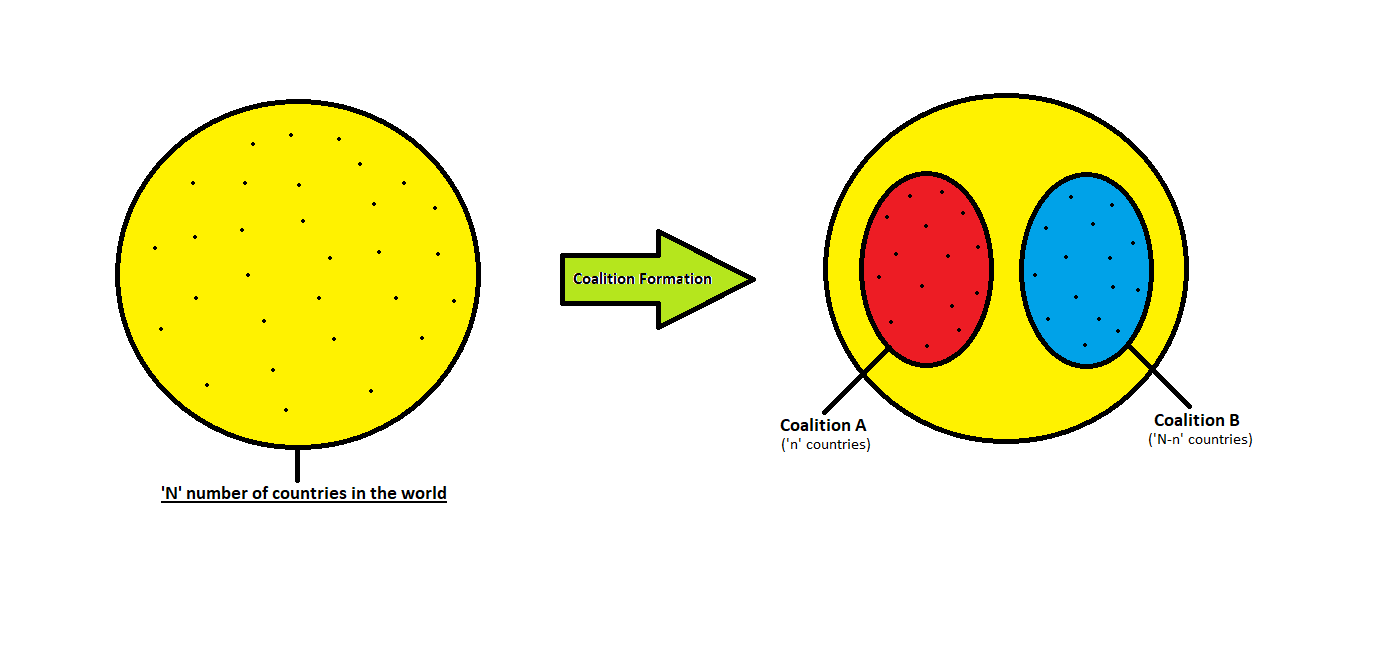
\includegraphics[width=1\linewidth]{Images/Coalition_Formation.png}
    \caption{Coalition Formation}
    \label{fig:}
\end{figure}


A coalition is a short-term association of people or groups that have different objectives. This means that for coalitions to work, there is no need to have a consensus on matters that are beyond the control of the coalition as there is normally little or no value in it. This makes power, or control over future decisions, a good basis for forming a coalition because it can be used to gain many different objectives and some of these may be conflicting. Although two members might have adversarial objective later on, the existing collaboration can enable them achieve a number of objectives that can be complimentary at that time. Politics is all about who gets what, when and how – and the ‘who’ is often defined in terms of power \cite{r6}.

Coalition building plays a significant role in international relationship and international politics. It influences countries’ strength, external and internal security, and they may achieve great power by cooperating and working together. In our model we have following assumptions: There are total N countries in the world. There are two coalition which are represented as coalition A and coalition B respectively. The military strength of ith country is represented as Ai. Coalition formation is a part in which an individual country will decide to join either coalition A or coalition B. The coalition formation may be depended on the various factors such as total military strength, Economic interests, Geographical positions and strategies, historical relationship etc. Let us assume that from total N countries, n countries join coalition A and (N-n) countries join coalition B. As the army of each country is Ai, the total military strength of coalitions can be demonstrated as below: (equations of army of coalition A and B)

Army of coalition A = number of countries in coalition A (n) * total number of army of each country i (\(A_i\)).

Army of coalition B = number of countries in coalition B (N-n) * total number of army of each country i (\(A_i\)).

\section{Stability Condition for Coalition's Payoff}

\begin{figure}[h]
    \centering
    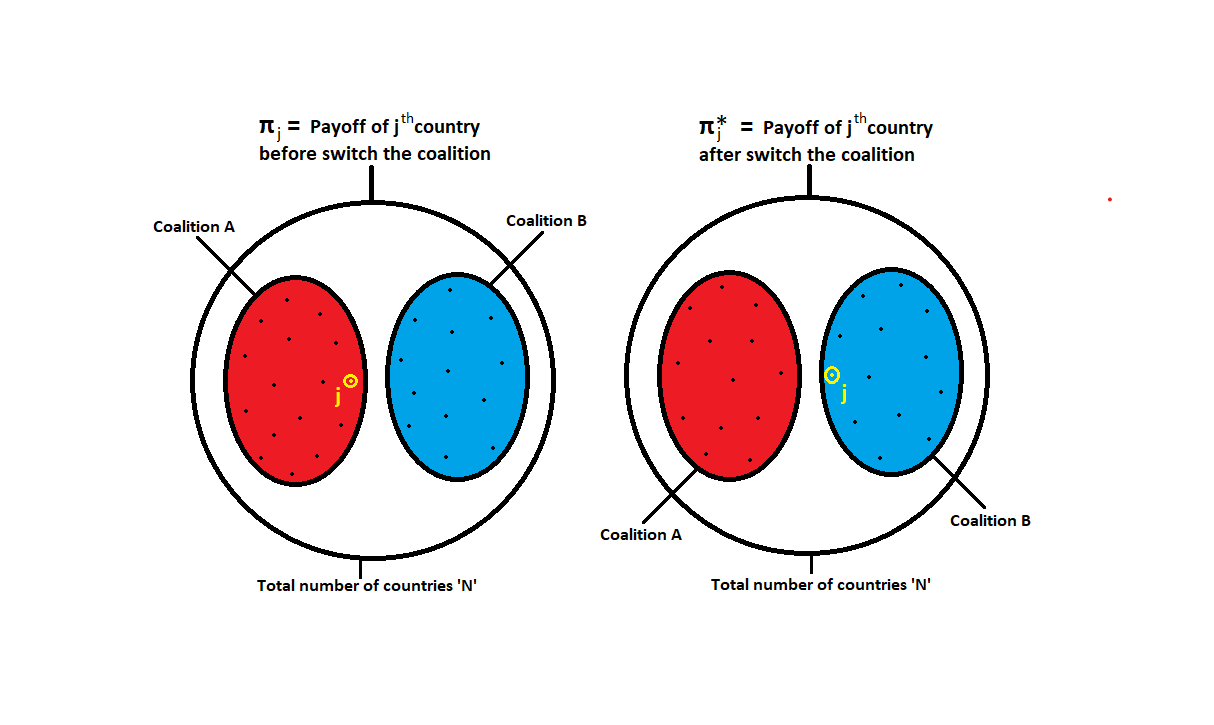
\includegraphics[width=1\textwidth]{Images/Payoff_stability.png}
    \caption{Payoff Stability Concept}
    \label{fig:2.1.1}
\end{figure}


\[
\pi\left(j, \{a_1, a_2, \ldots, j, \ldots ,a_n\}, \{b_1, b_2, \ldots, b_m\}\right)
\]

Here, $\pi$ denotes the payoff function for \(jth\) country in coalition A. where \(j\) is the country of coalition \(A\) and \(a_1, a_2, a_3, \ldots, a_n\) are all countries of coalition \(A\) and \(b_1, b_2, \ldots, b_m\) are countries of coalition \(B\).
\\[2em]
\textbf{Definition 2.1.0:} Coalition A is internally stable if and only if Coalition B is externally stable.

For every $a_j \in A$:

\begin{equation}
\begin{split}
\pi\left(a_j, \{a_1, a_2, \ldots, a_j, \ldots, a_n\}, \{b_1, b_2, \ldots, b_m\}\right) \\
\geq \pi^*\left(a_j, \{a_1, a_2, \ldots, a_{n-1}\}, \{a_j, b_1, b_2, \ldots, b_m\}\right)
\end{split}
\end{equation}

This above condition implies that no single \(a_j\) country of coalition A wants to leave their coalition for another coalition. Here, $\pi$ represents the payoff function for \(a_j\) country when they are in coalition A before it switches to coalition B. $\pi^*$ represents the payoff function for \(a_j\) country if they leave coalition A and join coalition B. The inequality indicates that \(a_j\) receives a higher or equal payoff by staying in coalition A than by leaving and joining coalition B. In this condition, no single \(a_j\) country outside of coalition B wants to join coalition B because they receive higher or equal payoff by staying in coalition A. If this condition holds then we can say that the coalition A is internally stable if and only if coalition B is externally stable.
\\[2em]
\textbf{Definition 2.1.1:} Coalition A is externally stable if and only if coalition B is internally stable.

 For every $b_j \in B$:

\begin{equation}
\begin{split}
\pi\left(b_j, \{a_1, a_2, \ldots, a_n\}, \{b_1, b_2, \ldots, b_j, \ldots, b_m\}\right) \\
\geq \pi^*\left(b_j, \{b_j, a_1, a_2, \ldots, a_n\}, \{b_1, b_2, \ldots, b_{m-1}\}\right)
\end{split}
\end{equation}

This above condition demonstrates that no single \(b_j\) country outside of coalition A wants to join coalition A. Here, $\pi$ represents the payoff function for \(b_j\) country when they are in coalition B whereas $\pi^*$ represents the payoff function for \(b_j\) if they leave coalition B and join coalition A. The inequality indicates that \(b_j\) country receives a higher or equal payoff by staying in coalition B than by leaving and joining coalition A. In this condition, no single \(b_j\) country of coalition B wants to leave their coalition for another coalition because they receive a higher or equal payoff by staying in coalition B than by leaving and joining coalition A. If this condition holds then we can say that the coalition A is externally stable if and only if the coalition B is internally stable. 

Internal stability demonstrates that no member of the coalition could profit from leaving the coalition. Each member concludes that remaining in the coalition is at least as helpful as leaving, both for themselves and their current partners.External stability indicates that the coalition members don't want to add any new members. This is because introducing a new member might have a detrimental influence on some of the existing members, increasing their payoff function \cite{r7} .


\newpage

\section{Mathematical Background}

\subsection{Derivation of Lanchester's Square Law}

Consider the differential equations describing the attrition rates of two opposing forces:

\begin{align}
    \frac{d A}{dt} &= -K_b B \\
    \frac{d B}{dt} &= -K_a A
\end{align}

To solve these, we use cross multiplication:

\begin{align}
    K_a A \frac{d A}{dt} &= K_b B \frac{d B}{dt}
\end{align}

Integrating both sides:

\begin{align}
    K_a \int A \frac{d A}{dt} \, dt &= K_b \int B \frac{d B}{dt} \, dt
\end{align}

We can express this as:

\begin{align}
    K_b \left( \frac{B^2}{2} + C \right) &= K_a \left( \frac{A^2}{2} + D \right)
\end{align}

Combining constants $C$ and $D$ into a single constant $E$:

\begin{align}
    K_b \frac{B^2}{2} - K_a \frac{A^2}{2} &= E
\end{align}

This above equation (3.8) is known as Lanchester Square Law.

Given initial conditions:

\begin{align}
    A = n \cdot A_i \\
    B = (N - n) \cdot A_i
\end{align}

Substituting in above equation
\begin{align}
    \frac{A_i^2}{2} \left[ K_b (N - n)^2 - K_a n^2 \right] &= E
\end{align}

For \(E = 0\),

\begin{align}
    K_b \frac{B^2}{2} - K_a \frac{A^2}{2} &= 0 \\
    B &= A \sqrt{\frac{K_a}{K_b}}
\end{align}

Putting initial conditions,

\begin{align}
    (N - n) \cdot A_i &= n \cdot A_i \sqrt{\frac{K_a}{K_b}} \\
    n = \frac{N} {\sqrt{\frac{K_a}{K_b}} + 1} 
\end{align}

This above equation (3.15) help to determine how the fraction of kill rate relates to number of countries in each coalition.


\newpage
\section{Geographical Demonstrates}

\begin{figure} [h]
    \centering
    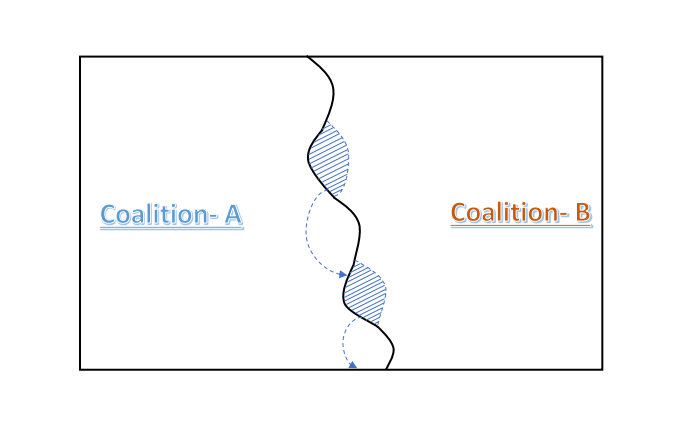
\includegraphics[width=1\linewidth]{Images/Geographical advantages.png}
    \caption{Geographical Demonstrates}
    \label{fig:2.1.2}
\end{figure}


This figure demonstrates the initial power and territorial balance in between Coalition A and Coalition B. This equality prevents either of them from achieving a vital advantage.  Nevertheless, this equilibrium can be disturbed in case one of the coalitions gets an advantage either by capturing strategically valuable areas of the other’s territory with military operations or by politically influencing the country from the other’s coalition to join their coalition. For instance, If Coalition-A acquires a region from Coalition-B that can be rich in resources or may have a geographical advantage then it not only achieves land but also escalates its resources and strategic position.

This newly acquired region is highlighted in shaded areas in the figure. Increment in Coalition-A’s resources would generate a power imbalance.  Accessory resources permit coalition-A to strengthen its military power and enhance its political impact which leads to making further conquests feasible. As the power of Coalition-A develops, Coalition-B finds it increasingly arduous to fortify its remaining territories. The increased capabilities of Coalition-A make following territorial expansions possible, gradually weakening Coalition-B. This cycle of conquest and resource gaining can eventually lead Coalition-A to prevail over the whole region, as demonstrated by the arrows showing Coalition-A’s territorial advancement.

Geographical research in this approach is meant to help locate critical areas that need to be politically controlled to strengthen a state’s power. This approach is known as the ‘geopolitical’ and it concentrates on strategy, nationalism and power. It views the international system as involving power and war and the objective of which is to attain primacy for a particular state. This power-oriented technique began in the late 20th century after the imperial strategies, state competitiveness, and the emergence of geography as a discipline. There are scholars who think that Herodotus was an actual spy of Athenian imperialism and the use of rationalization and ideology was a part of a covert plan \cite{r5}.

Geographers who research international relations have begun to delve into architecture. Today's political strategists, particularly Robert Kaplan, pay closer attention to classic geopolitics. Geography seeks to demonstrate why geographical conditions and physical reality are important. Thinking spatially involves recognizing the unreliable truth of location. To understand nation-state power and growth, we must consider geographical factors. This theory is critical for understanding resource conflicts and the growth of powerful states. It is apparent that in the twenty-first century, a nation's influence is determined by its massive riches and ability to acquire more resources \cite{r5}.

\newpage
\chapter{Results and Stability Analysis}

\begin{figure} [h]
    \centering
    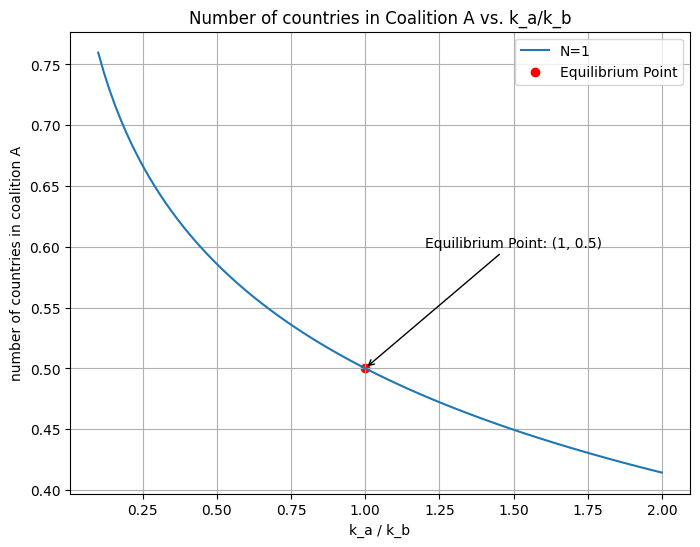
\includegraphics[width=0.75\linewidth]{Images/Stability points graph.png}
    \caption{Number of countries in coalition A vs kill rate}
    \label{fig:2.1.2}
\end{figure}

\newpage
\begin{table}[h]
\centering
\begin{tabular}{|c|c|}
\hline
$k_a/k_b$ & $n$ \\
\hline
0.25 & 0.67 \\
0.50 & 0.59 \\
0.75 & 0.54 \\
1.00 & 0.50 \\
1.25 & 0.47 \\
1.50 & 0.45 \\
1.75 & 0.43 \\
2.00 & 0.41 \\
\hline
\end{tabular}
\caption{Values of $k_a/k_b$ and $n$}
\label{tab:k_ak_b_n}
\end{table}


The graph shows that the number of countries in Coalition A decreases as the kill rate ratio \(k_a/k_b\) increases, there is an equilibrium where exactly half of the countries belong to Coalition A. This indicates a balanced scenario where the kill rates of the two coalitions are equal. That means all the points on the line which denotes stability points.

From the Geographical Demonstration, we analyze that Militaristic stable is always politically unstable because Militaristic governments may appear stable because the military maintains order, but they are essentially politically unstable. This is due to a lack of popular support, the prohibition of free elections and speech, and an over reliance on the military. If the military switches sides or there are problems within the military, the regime can rapidly disintegrate.

\chapter{Discussion}

\section{Mutually Assured Destruction}

Here, we are discussing about the situation when both coalition want to go for nuclear war.

\begin{table}[h!]
\centering
\begin{tabular}{c|c|c}
 & \textbf{Coalition B (Attack)} & \textbf{Coalition B (Not Attack)} \\
\hline
\textbf{Coalition A (Attack)} & $(-\infty, -\infty)$ & $(w, -\infty)$ \\
\hline
\textbf{Coalition A (Not Attack)} & $(-\infty, w)$ & $(1, 1)$ \\
\end{tabular}
\caption{Destruction Matrix for Coalition A and Coalition B}
\end{table}


If the both coalitions want to go for nuclear war, both suffer total destruction, leading to the worst possible outcome. This shows that nuclear war is highly undesirable for both coalitions due to its catastrophic consequences. If only one coalition attacks while the other does not, the attacking coalition suffers significant destruction (w) where, \( w < 1 \), while the non-attacking coalition faces no immediate destruction. This illustrates that while attacking may still result in substantial damage, it is less catastrophic compared to mutual destruction. The non-attacking party benefits from avoiding the direct consequences of war but does not gain anything. If both coalitions avoid attacking each other, both enjoy a stable and peaceful situation, with minimal positive outcomes (represented as 1). This highlights the value of avoiding nuclear conflict, as it leads to mutual benefit and prevents the severe consequences of war.

Building on the International Security Advisory Board's 2012 report, future work should explore the transition from Mutually Assured Destruction (MAD) to Mutually Assured Stability (MAS) by addressing five critical areas. Firstly, there should be a focus on managing the spread of technology facilitated by globalization, ensuring that advanced military capabilities do not fall into the hands of minor or threshold states. Secondly, further research should examine strategies to mitigate the incentives for preemptive strikes inherent in contemporary deterrence theory, particularly in light of ongoing technological advancements\cite{r4}.

Developing robust frameworks for international cooperation and transparency will be essential to counter the destabilizing effects of these advancements. Additionally, policy recommendations should aim at reducing surplus nuclear arsenals and preventing proliferation. Finally, establishing comprehensive security measures that adapt to the dynamic technological landscape will be crucial for sustaining global nuclear stability and preventing conflict. These efforts will contribute to a more secure and balanced international order, addressing the limitations of the MAD doctrine in the modern era\cite{r4} .

Mutually Assured Stability (MAS) is a status where Russia cannot overpower or threaten the United States or vice versa using a first strike or coercion to be able to respond or negotiate or bargain. It expands upon the concept of ‘strategic stability’ from the twentieth century to try to address the new technologies and security issues more effectively. MAS includes such mechanisms as arms control treaties, conveying of military information, and communication to limit the possession of nuclear weapons and to avoid situations when one side may prepare for an attack due to lack of other information. It is to achieve the spirit of protection through strong, effective agreements and coordination; thus making the relations between Russia and the U. S. stronger and safer in the 21st century \cite{r9}.

\chapter{Conclusion}

This study explores the application of the Lanchester model in the context of coalition formation, with a particular focus on the dynamics of internal and external stability between two competing coalitions. By applying Lanchester's Linear and Square Laws, we provide a mathematical framework to analyze combat dynamics and the influence of various factors on coalition performance. Key parameters such as kill rates, synergy effects, and stability conditions are examined to understand the intricacies of coalition formation and outcomes.

The findings indicate that the balance of power plays a crucial role in the interactions between coalitions. The study demonstrates that a coalition's internal stability is achieved when no member can profit from leaving the coalition, while external stability is maintained when the coalition is resistant to the addition of new members from opposing forces. The equilibrium condition, where exactly half of the countries belong to each coalition, highlights a balanced scenario with equal kill rates, representing stability points.

Furthermore, the research incorporates geopolitical considerations, emphasizing the significance of geographical advantages in coalition dynamics. The acquisition of strategic territories and resources by one coalition can disrupt the balance of power, leading to potential dominance over the opposition. Here, We can conclude that militaristic stable is always politically unstable.

In the broader context of international relations, the study discusses the implications of Mutually Assured Destruction (MAD) and the potential for transitioning to Mutually Assured Stability (MAS). The analysis underscores the catastrophic consequences of nuclear warfare and the need for robust international cooperation and transparency to prevent conflict and ensure global stability.

Overall, this study provides a comprehensive understanding of coalition formation using the Lanchester model, offering valuable insights into the factors influencing coalition stability and performance. The integration of mathematical modeling and geopolitical analysis contributes to a deeper comprehension of strategic interactions in international politics.

%\printbibliography
\bibliographystyle{unsrt}
\bibliography{bibfile.bib}

\end{document}